\section{Diseño de software} \label{sec:dis}
% (estático e dinámico) ou do hardware: indicaranse os aspectos máis relevantes correspondentes ao deseño do traballo realizado
% estatico -> diagrama de clases
% dinamico -> diagrama de secuencia

    \begin{figure}[h!]
    \centering
        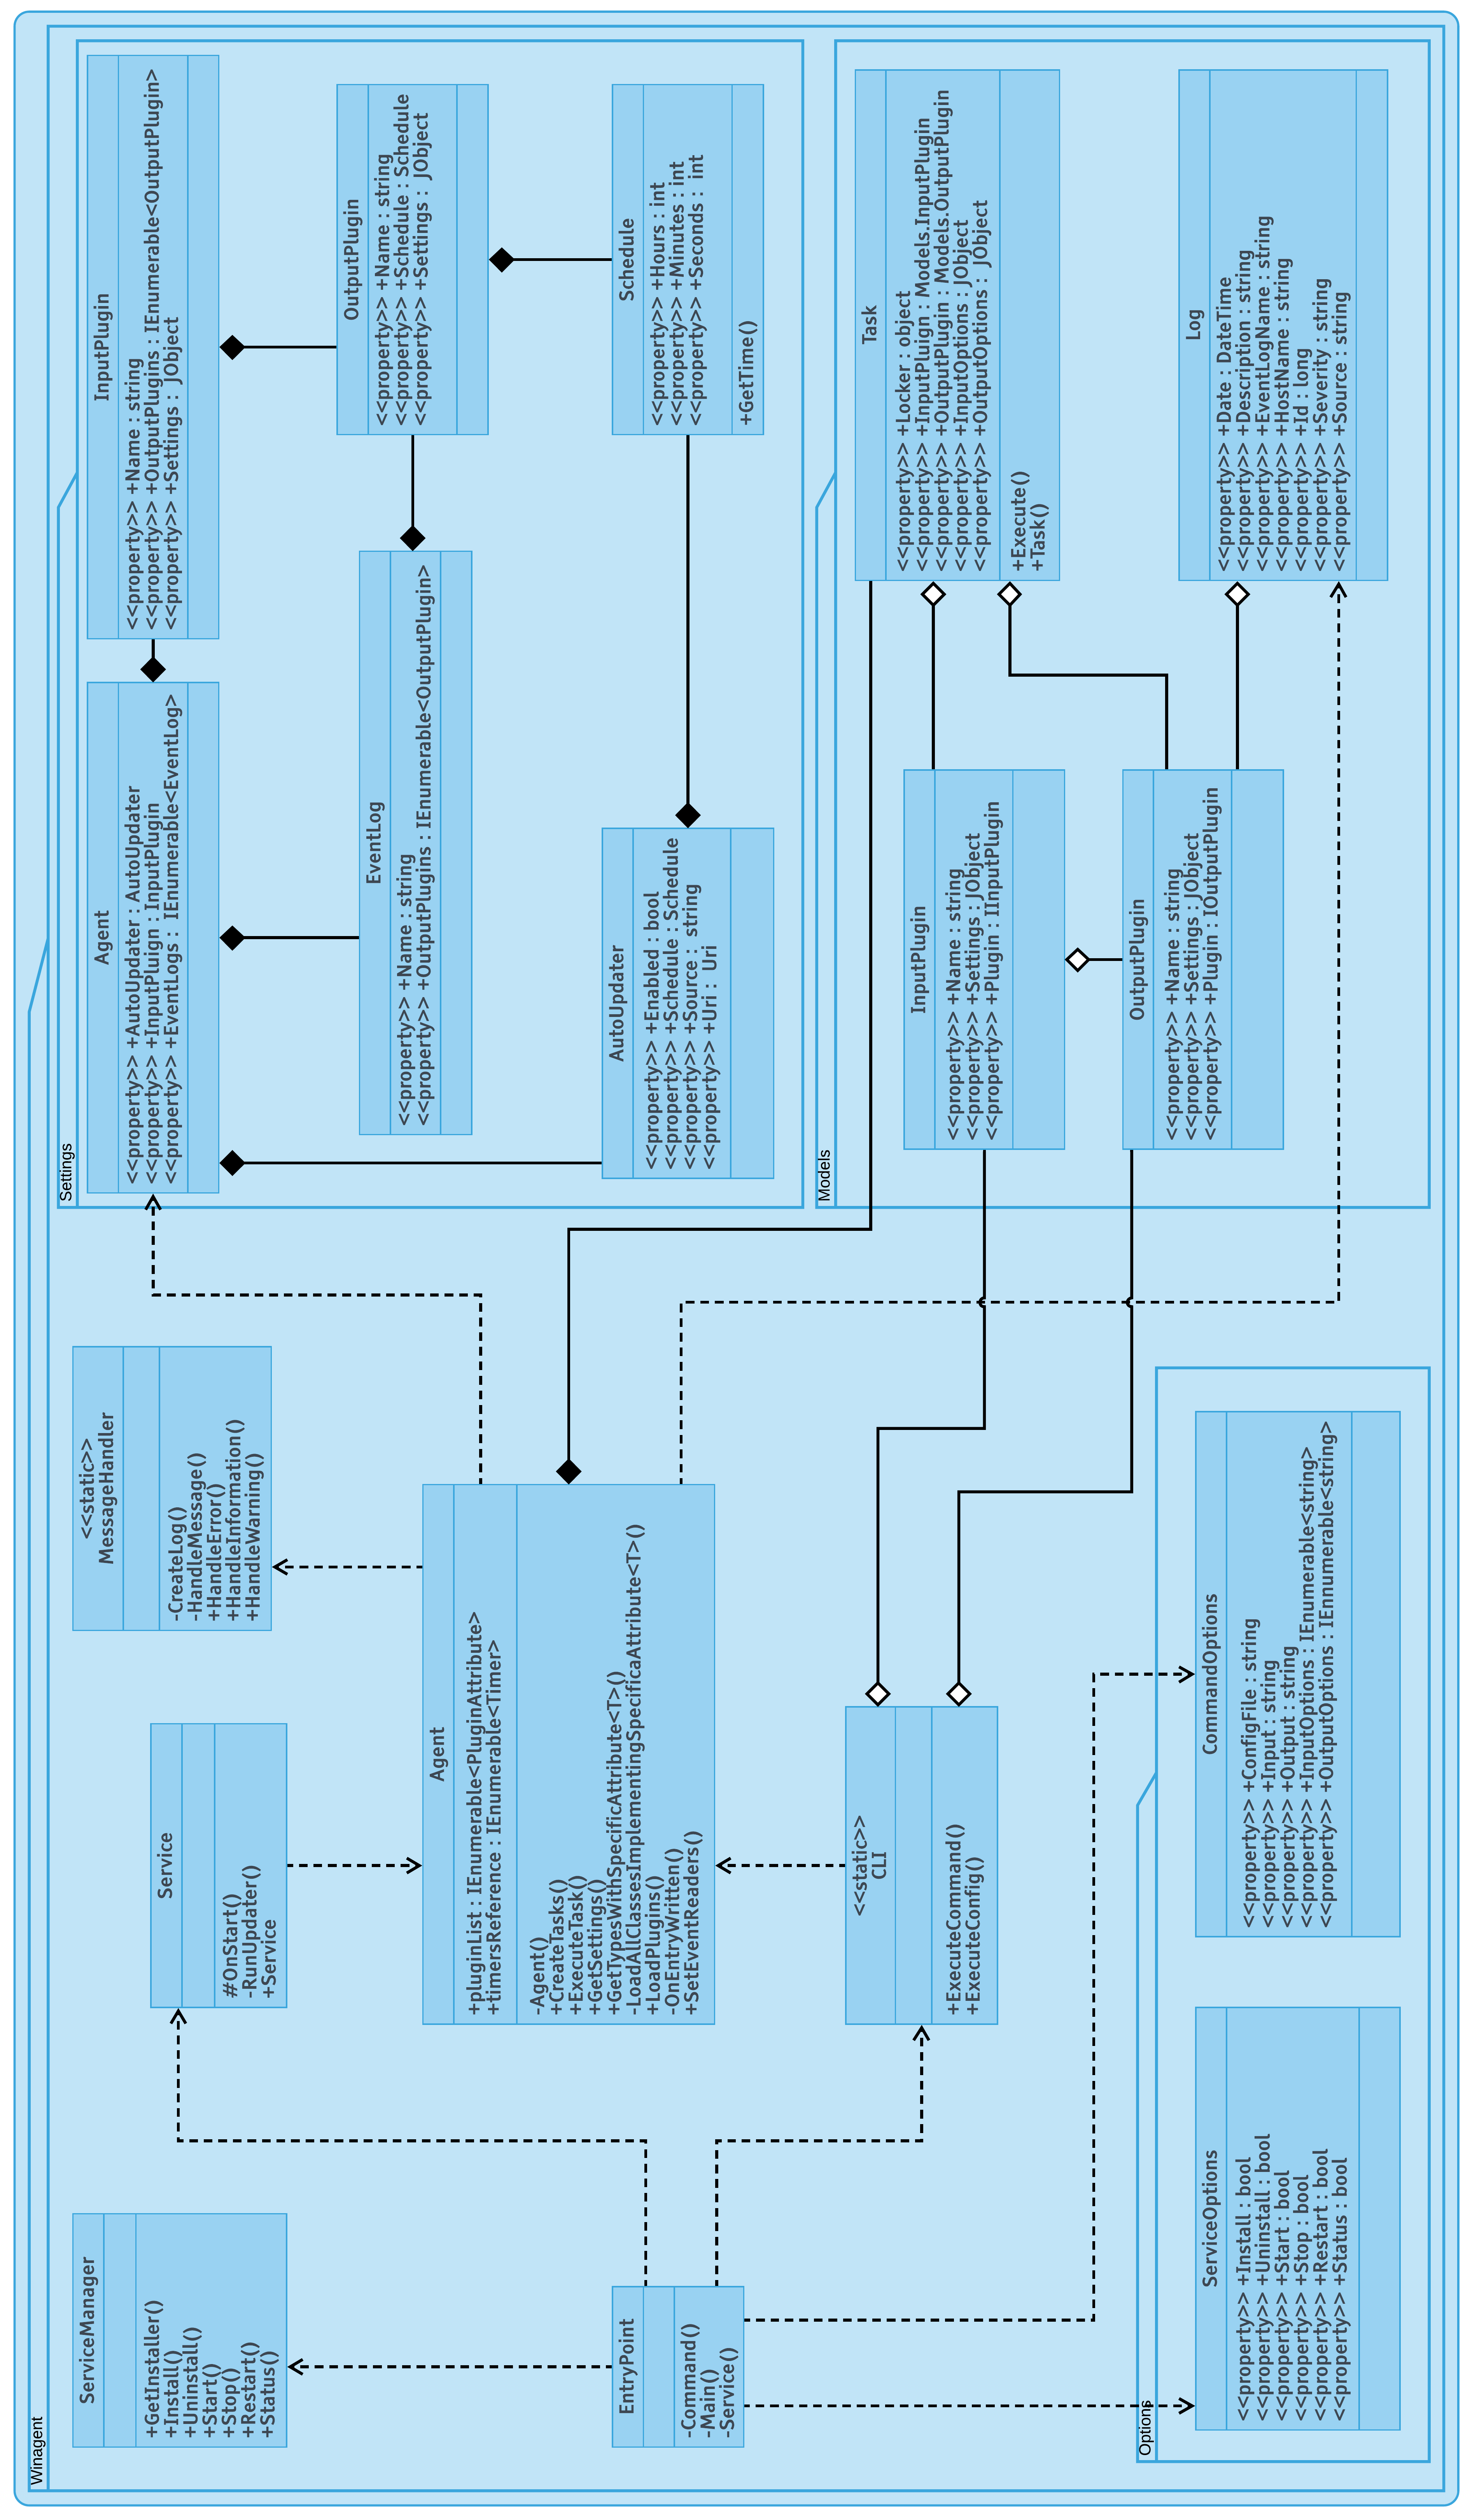
\includegraphics[scale=0.138]{diagrama-de-clases.png}
        \caption{Diagrama de clases}
        \label{fig:class-diagram}
    \end{figure}

    \begin{figure}[h!]
    \centering
        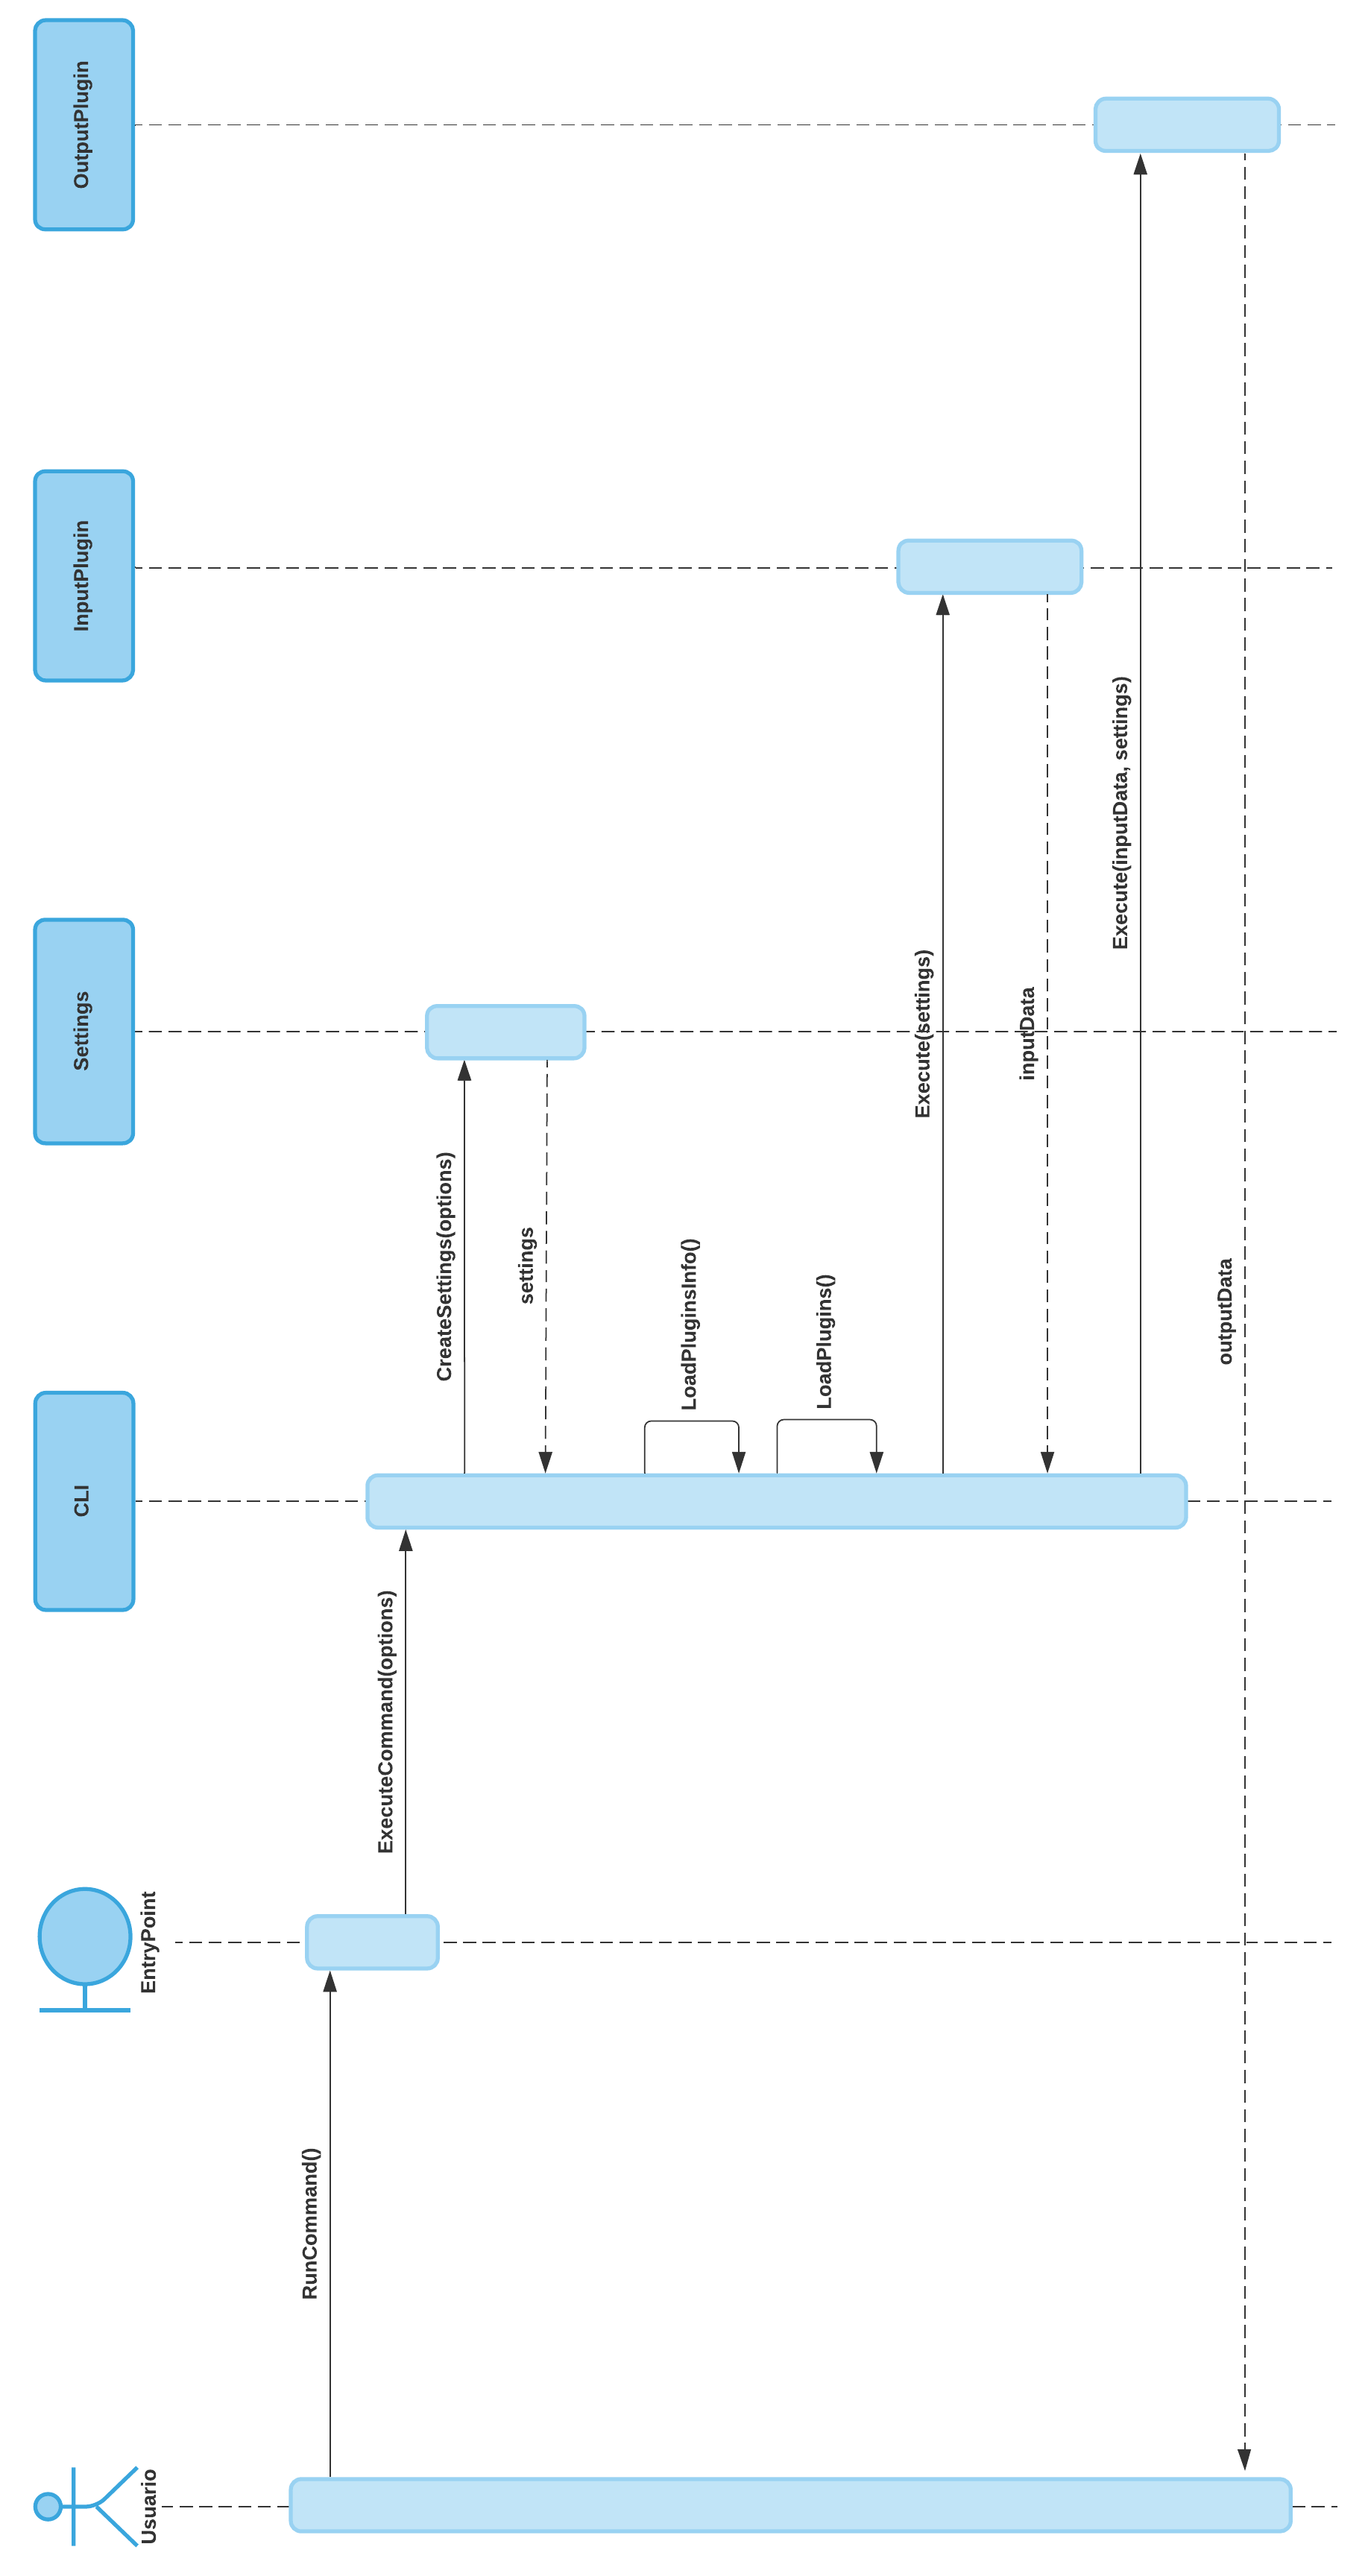
\includegraphics[scale=0.25]{diagrama-secuencia-cli.png}
        \caption{Diagrama de secuencia - \textit{CLI}}
        \label{fig:sequence-diagram-cli}
    \end{figure}
    
    \begin{figure}[h!]
    \centering
        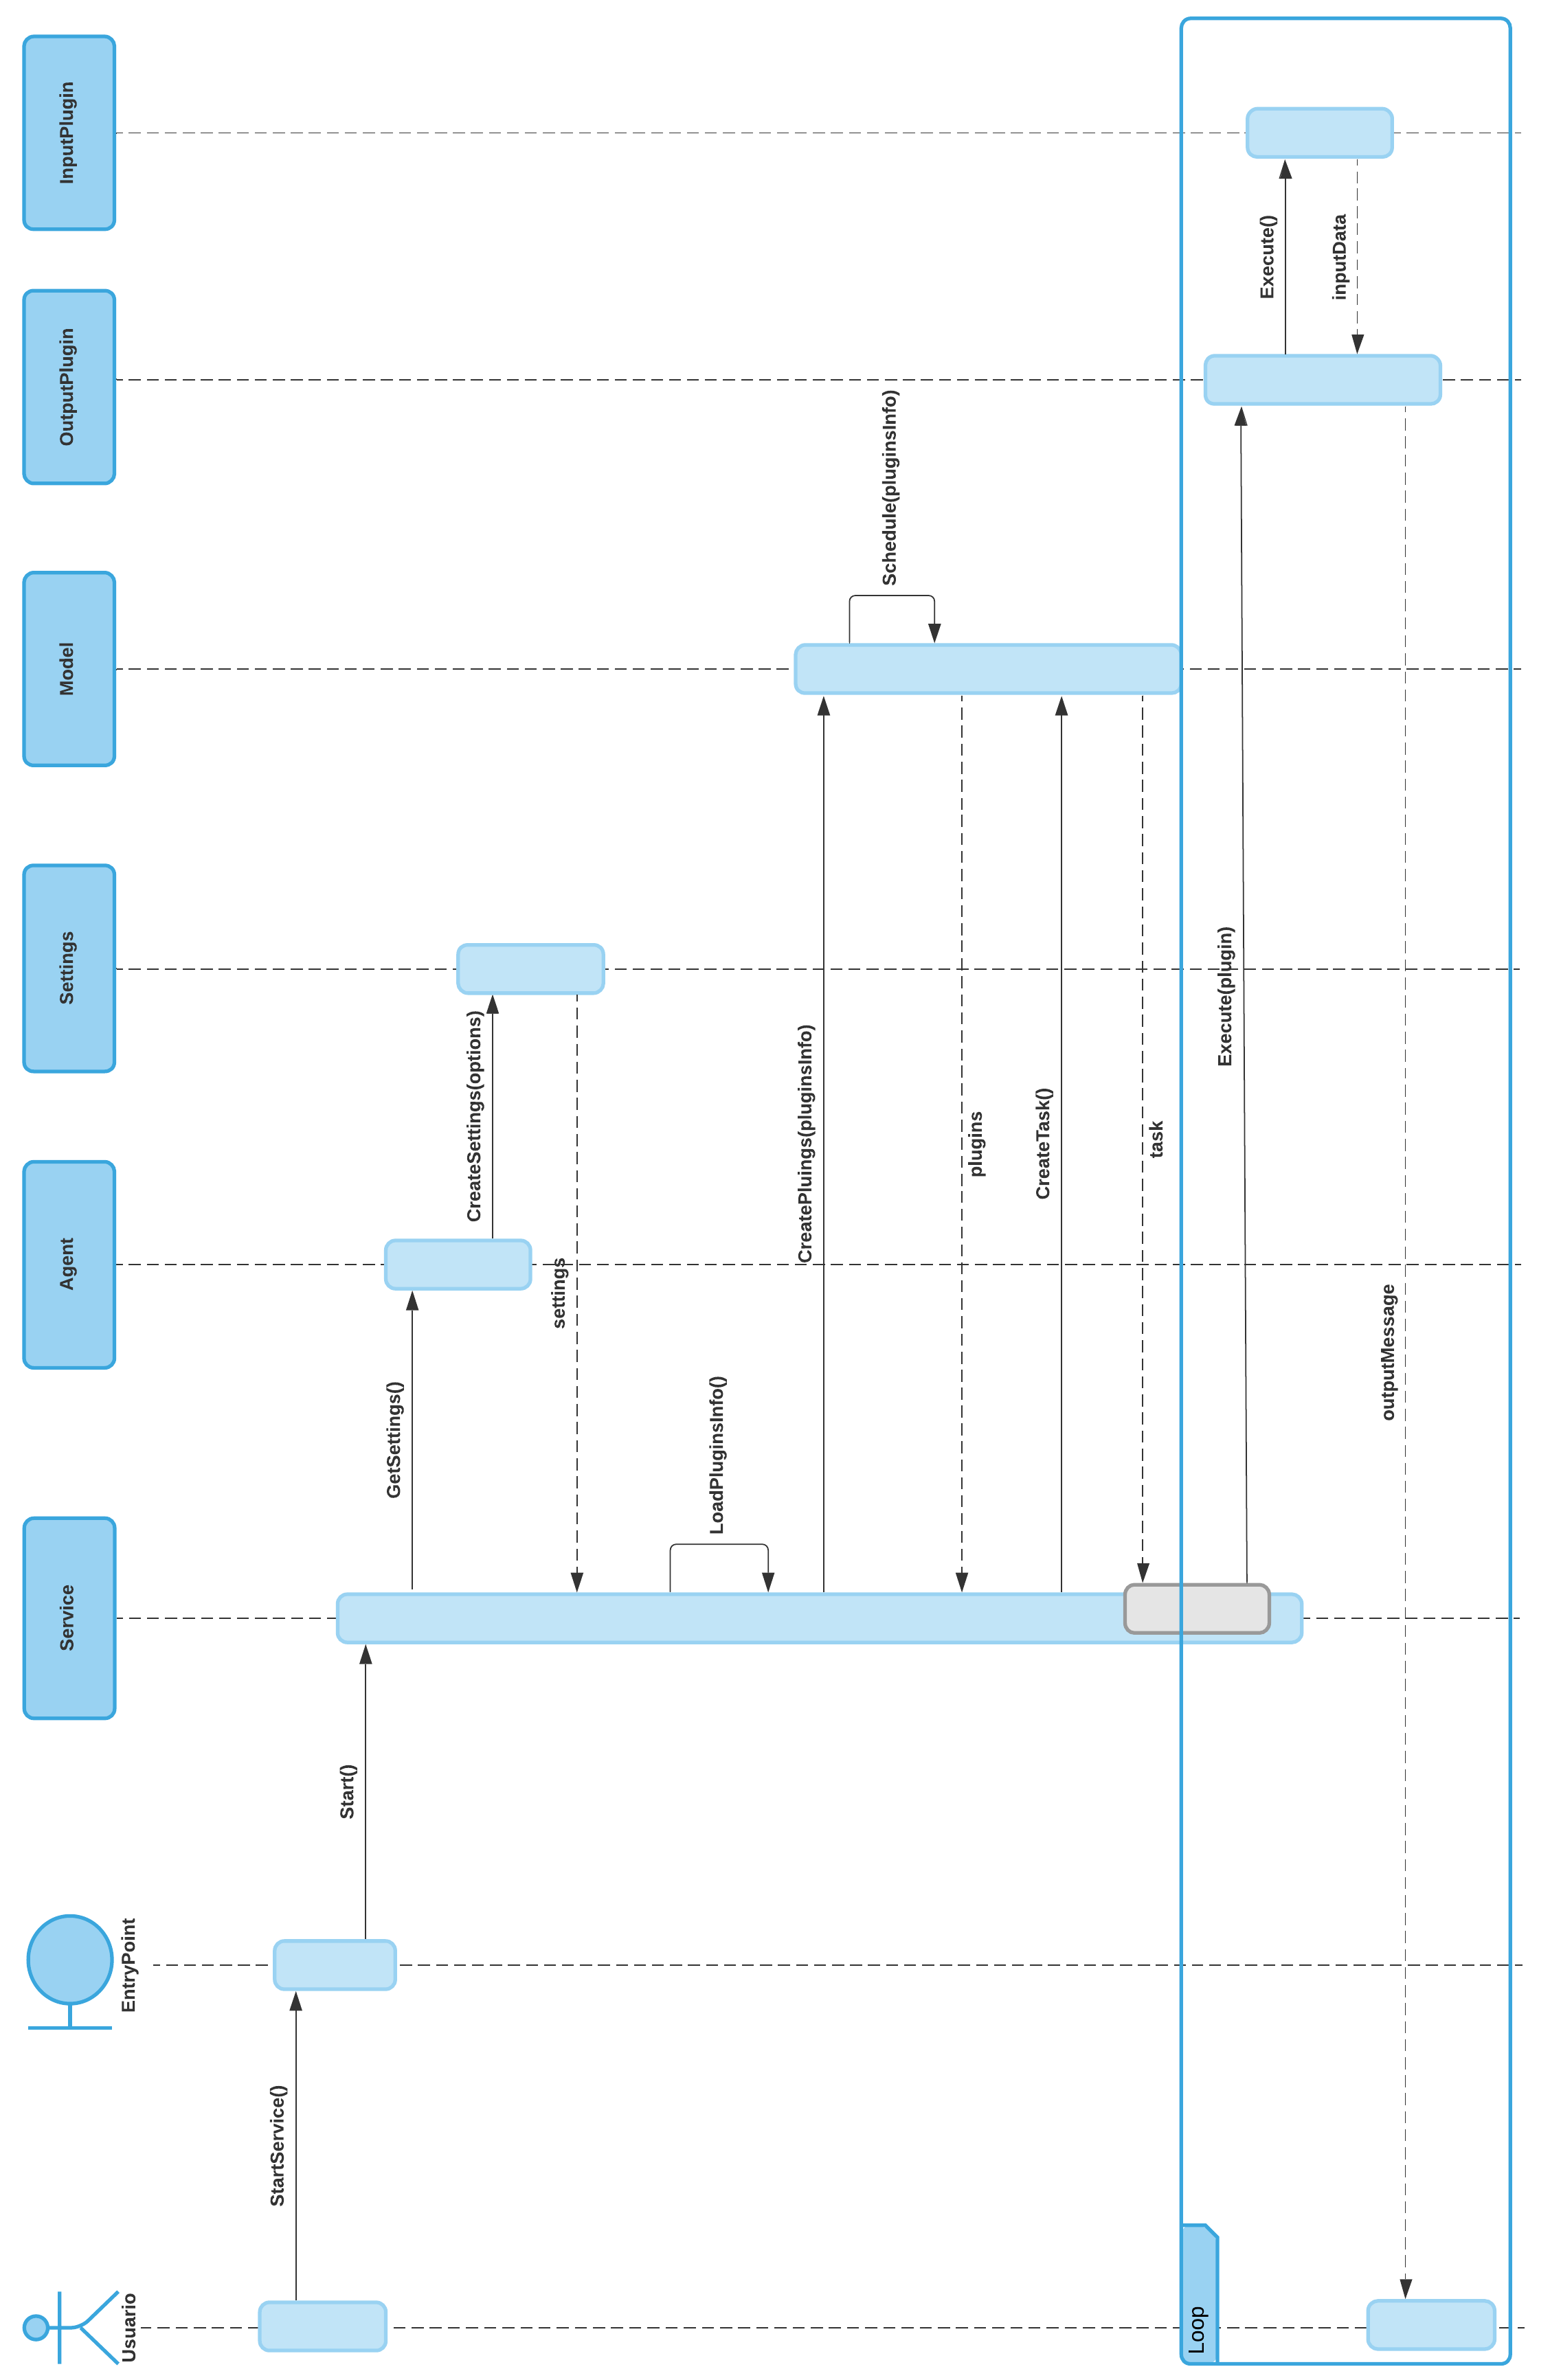
\includegraphics[scale=0.25]{diagrama-secuencia-servicio.png}
        \caption{Diagrama de secuencia - Servicio}
        \label{fig:sequence-diagram-service}
    \end{figure}